\documentclass[a4paper]{article}
\usepackage[utf8]{inputenc}
\usepackage[fleqn]{amsmath}
\usepackage{amssymb}
\usepackage{mathtools}
\usepackage{amsfonts}
\usepackage{lastpage}
\usepackage{tikz}
\usepackage{float}
\usepackage{textcomp}
\usetikzlibrary{patterns}
\usepackage{pdfpages}
\usepackage{gauss}
\usepackage{fancyvrb}
\usepackage[table]{colortbl}
\usepackage{fancyhdr}
\usepackage{graphicx}
\usepackage[margin=2.5 cm]{geometry}

\definecolor{listinggray}{gray}{0.9}
\usepackage{listings}
\lstset{
    language=,
    literate=
        {æ}{{\ae}}1
        {ø}{{\o}}1
        {å}{{\aa}}1
        {Æ}{{\AE}}1
        {Ø}{{\O}}1
        {Å}{{\AA}}1,
    backgroundcolor=\color{listinggray},
    tabsize=3,
    rulecolor=,
    basicstyle=\scriptsize,
    upquote=true,
    aboveskip={0.2\baselineskip},
    columns=fixed,
    showstringspaces=false,
    extendedchars=true,
    breaklines=true,
    prebreak =\raisebox{0ex}[0ex][0ex]{\ensuremath{\hookleftarrow}},
    frame=single,
    showtabs=false,
    showspaces=false,
    showlines=true,
    showstringspaces=false,
    identifierstyle=\ttfamily,
    keywordstyle=\color[rgb]{0,0,1},
    commentstyle=\color[rgb]{0.133,0.545,0.133},
    stringstyle=\color[rgb]{0.627,0.126,0.941},
  moredelim=**[is][\color{blue}]{@}{@},
}

\lstdefinestyle{base}{
  emptylines=1,
  breaklines=true,
  basicstyle=\ttfamily\color{black},
}

\pagestyle{fancy}
\def\checkmark{\tikz\fill[scale=0.4](0,.35) -- (.25,0) -- (1,.7) -- (.25,.15) -- cycle;}
\newcommand*\circled[1]{\tikz[baseline=(char.base)]{
            \node[shape=circle,draw,inner sep=2pt] (char) {#1};}}
\newcommand*\squared[1]{%
  \tikz[baseline=(R.base)]\node[draw,rectangle,inner sep=0.5pt](R) {#1};\!}
\newcommand{\comment}[1]{%
  \text{\phantom{(#1)}} \tag{#1}}
\cfoot{Page \thepage\ of \pageref{LastPage}}
\DeclareGraphicsExtensions{.pdf,.png,.jpg}
\author{Nikolaj Dybdahl Rathcke (rfq695) \\ Victor Petrèn Bach Hansen (grn762)}
\title{Advanced Computer Systems \\ Assignment 4}
\lhead{Advanced Computer System}
\rhead{Assignment 4}

\begin{document}
\maketitle

\section{Recovery Concepts}
\subsection{Force, no-steal approach}
By implementing a no-steal approach, there is no need to undo changes of aborted transactions as they haven't been written to disk. By implementing a force approach, we know the changes have been written to disk at commit time, thus there is no need to redo commited transactions.
\subsection{Stable storage vs. nonvolatile storage}
Both stable nonvolatile storage ensures atomicity and durability of commited transactions when a system crash occurs, but nonvolatile storage has no guarantee of these properties in the event of media failure. The advantage of stable storage is that it survives both system crashes and media failures, as it maintains multiple copies of information on nonvolatile storage.
\subsection{}
The first situation where the log tail is forced to stabe storage, is when a transaction is commited, whether or not you are using a force or no-force approach. The second situation is before writing a page to disk, all update log records that describes a change to this page, must be forced to stable storage.

Log forces are necessary in order to maintain durability by ensuring that records of all changes to the database is available on stable storage, as we attempt to recover from a crash. If there were no records of these changes, we would not be able to ensure that changes of a commited transaction would survive a crash.

\section{ARIES}
\subsection{}
The resulting transaction table after the analysis will look like:
\begin{center}
\begin{tabular}{c|c|c}
  TRX ID & LAST LSN & STATUS \\
  \hline
  T1 & 4 & active \\
  \hline
  T2 & 9 & active \\
\end{tabular}
\end{center}
And the dirty page table will be:
\begin{center}
\begin{tabular}{c|c}
  PAGE ID & REC LSN \\
  \hline
  P1 & 4 \\
  \hline
  P2 & 3 \\
  \hline
  P3 & 6 \\
  \hline
  P5 & 5
\end{tabular}
\end{center}
where the REC LSN (or recLSN) is the smallest LSN for a page that occurs between the last checkpoint and the crash.

\subsection{}
Winners are the transactions that has commited since the checkpoint, while losers are those that have not and are considered aborted. Therefore the set of winner is $\{T3\}$ and the losers is the set $\{T1, T2\}$.

\subsection{}
The REDO phase starts on LSN $3$, as this is the smallest recLSN. The undo phase ends in LSN $3$ as well, as $T1$ is the last loser transaction to be undone (descending number of LSN).

\subsection{}
The log records that may be rewritten is the set of LSN $\{3, 4, 5, 6\}$, since these are ones that fullfill the criteria: Being in the dirty page table, have recLSN $\leq$ LSN and having pageLSN $<$ LSN.

\subsection{}
The log records that are undone is the set of LSN $\{9, 8, 5, 4, 3\}$ since these are records of the loser transaction that has made an update.

\subsection{}
The content log will be:
\begin{verbatim}
            LSN  LAST_LSN  TRAN_ID  PAGE_ID  TYPE
          ---  --------  -------  -------  -------
          1    -         -        -        begin CKPT
          2    -         -        -        end CKPT
          3    NULL      T1       P2       update
          4    3         T1       P1       update
          5    NULL      T2       P5       update
          6    NULL      T3       P3       update
          7    6         T3       -        commit
          8    5         T2       P5       update
          9    8         T2       P3       update
          10   6         T3       -        end

          -------------- CRASH ------------------

          12   -         T2       P3       CLR: Undo LSN 9
          13   -         T2       P5       CLR: Undo LSN 8
          14   -         T2       P5       CLR: Undo LSN 5
          15   13        T2       -        end
          16   -         T1       P1       CLR: Undo LSN 4
          17   -         T1       P2       CLR: Undo LSN 3
          18   16        T1       -        end
\end{verbatim}
The undo changes are done in "reverse" order. When we undo a log entry that has \texttt{LAST\_LSN} set to \texttt{NULL}, we end the transaction in this entry.

\section{Questions for Discussion on the Performance Measurements}
\subsection{}
The book generations are performed by making a random book with ISBN $1\leq ISBN\leq 1000$. Author and title has the same name as the ISBN. The number of copies we make is a random in the range $[50, 150)$ and we say it is an editor pick each time as one of the tests rely on this. \\
  For testing throughput and latency, we used $x$ workers where $x\in \{5,10,15,20,25,30\}$ (as larger was problematic when running on different address space). Each time we ensured that the number of \texttt{runFrequentBookStoreInteraction} is between $50$ and $70$ percent of all interaction for each worker. We also made sure that the workers had $99$ percent successfull interactions - otherwise they would not be counted in the calculations. \\
  Each worker did $100$ actual runs with $20$ warmup runs. Throughput was calculated for each worker and accumulated in a total throughput. This is almost the same as measuring the total of successfull interaction over the time it takes for an average worker to finish. This can kinda simulate what the throughput is in real time, though they do not run perfectly in parallel, so the throughput in real time would be a little lower. The other alternative was compute for CPU time, but since we want measure the advantage of running it with multiple threads, that calculation would defeat the purpose. Latency was calculated by getting the total number of successfull interaction and divide it by the total elapsed CPU time to estimate the average for a single interaction. \\
The experiment was run several times to be sure we got consistent results and one run of the experiment was used. The results were very alike, which is why we did not take an average.\\
The hardware used was a $4$-core Intel(R) Core(TM) i5-2520M CPU @ 2.50GHz with $16$GB of RAM.

\subsection{}
The following plots were obtained by running with actual runs set to $100$ and warmup runs set to $20$ as the tests done in different address space was too slow otherwise. The following plot compares the two measurement in terms of throughput:
\begin{figure}[H]
  \centering
  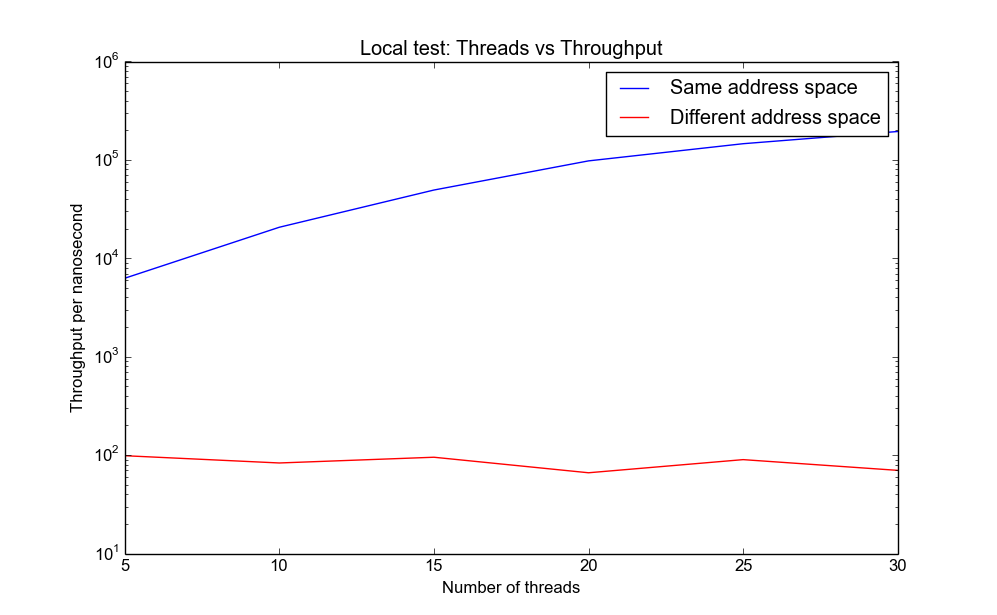
\includegraphics[scale=0.5]{fig1}
  \caption{Plot showing the correlation between number of threads and the throughput}
\end{figure}
The plot uses a logarithmic $y$-scale to better show the relation between the two. When the test were completed in the same adress space, we had a much higher throughput which is what we would expect. The thread/throughput correlation is almost linear while it is a bit more imprecise when done in different address space. \\
The other figure shows the relation in terms of latency:
\begin{figure}[H]
  \centering
  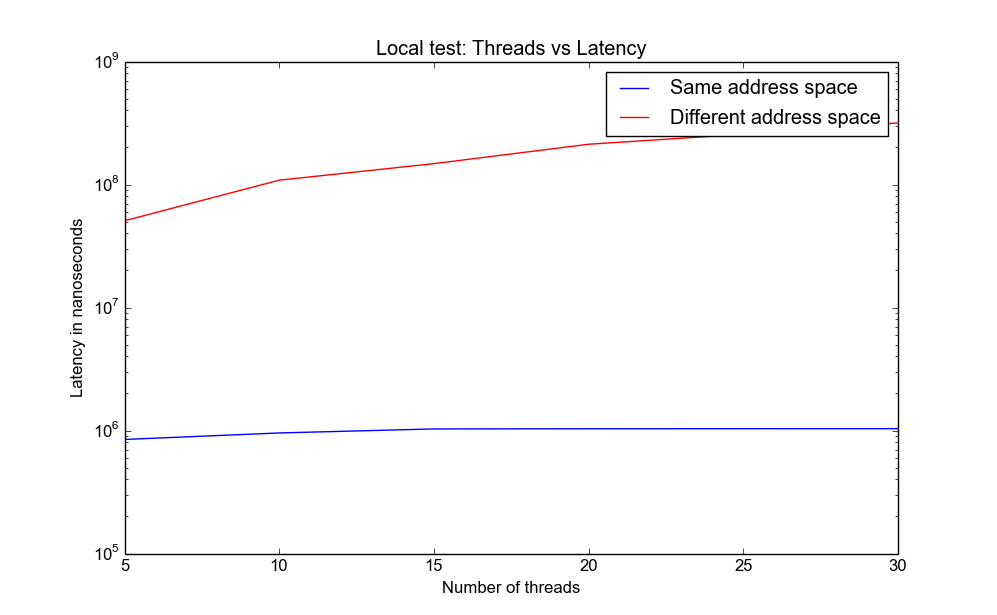
\includegraphics[scale=0.5]{fig2}
  \caption{Plot showing the correlation between the number of threads and latency}
\end{figure}
Again the latency is larger when run in different address space as we would have expected. It is also increasing when we increase the number of threads. When run in the same address space, it increases but seems to converge. However, we have only measured in $6$ points, so these are just observations.

\subsection{}
Throughput, or more precisely the goodput, is a good choice of metric for a bookstore. We want
to be able to process as many client as possible as fast as possible. Throughput also relates
to efficiency, so the more clients we process the better we can say our system is. The goodput
'ratio' also provides an indication of how well the system behaves. We can have high goodput,
while we still have many interactions that are unsuccessfull and this is not what we want.
Latency is also important in the sense that faster response times will mean we can obtain a higher throughput. So the two metrics are quite reliable for predicting the performance of the system. \\
While the two metrics we tested are desirable for testing the effectiveness of the system, we might also want to look at scalability of the system. How well it will handle a heavier and heavier workload. We might also want to look at the utilization of the computer resources we have.

\end{document}
